\documentclass[12pt,fleqn]{article}
\setlength{\parindent}{0pt}
\usepackage{graphicx}
\usepackage{cancel}
\usepackage{listings}
\usepackage[latin5]{inputenc}
\usepackage{color}
\setlength{\parskip}{8pt}
\setlength{\parsep}{0pt}
\setlength{\headsep}{0pt}
\setlength{\topskip}{0pt}
\setlength{\topmargin}{0pt}
\setlength{\topsep}{0pt}
\setlength{\partopsep}{0pt}
\setlength{\mathindent}{0cm}
\usepackage{showkeys}
\renewcommand*\showkeyslabelformat[1]{(#1)}

\begin{document}
Ders 18

Cift Entegrallerde Degisken Degisimi 

Ornek 

Bir elipsin alanini bulmak istedigimizi dusunelim. 

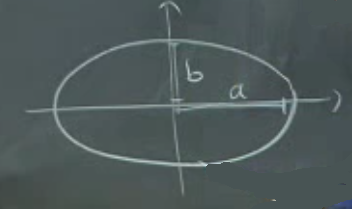
\includegraphics[height=2cm]{18_1.png}



\end{document}
